\documentclass[twoside]{book}

% Packages required by doxygen
\usepackage{fixltx2e}
\usepackage{calc}
\usepackage{doxygen}
\usepackage[export]{adjustbox} % also loads graphicx
\usepackage{graphicx}
\usepackage[utf8]{inputenc}
\usepackage{makeidx}
\usepackage{multicol}
\usepackage{multirow}
\PassOptionsToPackage{warn}{textcomp}
\usepackage{textcomp}
\usepackage[nointegrals]{wasysym}
\usepackage[table]{xcolor}

% Font selection
\usepackage[T1]{fontenc}
\usepackage[scaled=.90]{helvet}
\usepackage{courier}
\usepackage{amssymb}
\usepackage{sectsty}
\renewcommand{\familydefault}{\sfdefault}
\allsectionsfont{%
  \fontseries{bc}\selectfont%
  \color{darkgray}%
}
\renewcommand{\DoxyLabelFont}{%
  \fontseries{bc}\selectfont%
  \color{darkgray}%
}
\newcommand{\+}{\discretionary{\mbox{\scriptsize$\hookleftarrow$}}{}{}}

% Page & text layout
\usepackage{geometry}
\geometry{%
  a4paper,%
  top=2.5cm,%
  bottom=2.5cm,%
  left=2.5cm,%
  right=2.5cm%
}
\tolerance=750
\hfuzz=15pt
\hbadness=750
\setlength{\emergencystretch}{15pt}
\setlength{\parindent}{0cm}
\setlength{\parskip}{3ex plus 2ex minus 2ex}
\makeatletter
\renewcommand{\paragraph}{%
  \@startsection{paragraph}{4}{0ex}{-1.0ex}{1.0ex}{%
    \normalfont\normalsize\bfseries\SS@parafont%
  }%
}
\renewcommand{\subparagraph}{%
  \@startsection{subparagraph}{5}{0ex}{-1.0ex}{1.0ex}{%
    \normalfont\normalsize\bfseries\SS@subparafont%
  }%
}
\makeatother

% Headers & footers
\usepackage{fancyhdr}
\pagestyle{fancyplain}
\fancyhead[LE]{\fancyplain{}{\bfseries\thepage}}
\fancyhead[CE]{\fancyplain{}{}}
\fancyhead[RE]{\fancyplain{}{\bfseries\leftmark}}
\fancyhead[LO]{\fancyplain{}{\bfseries\rightmark}}
\fancyhead[CO]{\fancyplain{}{}}
\fancyhead[RO]{\fancyplain{}{\bfseries\thepage}}
\fancyfoot[LE]{\fancyplain{}{}}
\fancyfoot[CE]{\fancyplain{}{}}
\fancyfoot[RE]{\fancyplain{}{\bfseries\scriptsize Generated by Doxygen }}
\fancyfoot[LO]{\fancyplain{}{\bfseries\scriptsize Generated by Doxygen }}
\fancyfoot[CO]{\fancyplain{}{}}
\fancyfoot[RO]{\fancyplain{}{}}
\renewcommand{\footrulewidth}{0.4pt}
\renewcommand{\chaptermark}[1]{%
  \markboth{#1}{}%
}
\renewcommand{\sectionmark}[1]{%
  \markright{\thesection\ #1}%
}

% Indices & bibliography
\usepackage{natbib}
\usepackage[titles]{tocloft}
\setcounter{tocdepth}{3}
\setcounter{secnumdepth}{5}
\makeindex

% Hyperlinks (required, but should be loaded last)
\usepackage{ifpdf}
\ifpdf
  \usepackage[pdftex,pagebackref=true]{hyperref}
\else
  \usepackage[ps2pdf,pagebackref=true]{hyperref}
\fi
\hypersetup{%
  colorlinks=true,%
  linkcolor=blue,%
  citecolor=blue,%
  unicode%
}

% Custom commands
\newcommand{\clearemptydoublepage}{%
  \newpage{\pagestyle{empty}\cleardoublepage}%
}

\usepackage{caption}
\captionsetup{labelsep=space,justification=centering,font={bf},singlelinecheck=off,skip=4pt,position=top}

%===== C O N T E N T S =====

\begin{document}

% Titlepage & ToC
\hypersetup{pageanchor=false,
             bookmarksnumbered=true,
             pdfencoding=unicode
            }
\pagenumbering{alph}
\begin{titlepage}
\vspace*{7cm}
\begin{center}%
{\Large Gestion de courses }\\
\vspace*{1cm}
{\large Generated by Doxygen 1.8.13}\\
\end{center}
\end{titlepage}
\clearemptydoublepage
\pagenumbering{roman}
\tableofcontents
\clearemptydoublepage
\pagenumbering{arabic}
\hypersetup{pageanchor=true}

%--- Begin generated contents ---
\chapter{Hierarchical Index}
\section{Class Hierarchy}
This inheritance list is sorted roughly, but not completely, alphabetically\+:\begin{DoxyCompactList}
\item C\+I\+\_\+\+Model\begin{DoxyCompactList}
\item \contentsline{section}{Shop\+List\+\_\+model}{\pageref{class_shop_list__model}}{}
\item \contentsline{section}{Shopping\+List\+\_\+model}{\pageref{class_shopping_list__model}}{}
\item \contentsline{section}{User\+\_\+model}{\pageref{class_user__model}}{}
\end{DoxyCompactList}
\end{DoxyCompactList}

\chapter{Data Structure Index}
\section{Data Structures}
Here are the data structures with brief descriptions\+:\begin{DoxyCompactList}
\item\contentsline{section}{\hyperlink{class_shop_list__model}{Shop\+List\+\_\+model} }{\pageref{class_shop_list__model}}{}
\item\contentsline{section}{\hyperlink{class_shopping_list__model}{Shopping\+List\+\_\+model} }{\pageref{class_shopping_list__model}}{}
\item\contentsline{section}{\hyperlink{class_user__model}{User\+\_\+model} }{\pageref{class_user__model}}{}
\end{DoxyCompactList}

\chapter{Data Structure Documentation}
\hypertarget{class_shop_list__model}{}\section{Shop\+List\+\_\+model Class Reference}
\label{class_shop_list__model}\index{Shop\+List\+\_\+model@{Shop\+List\+\_\+model}}
Inheritance diagram for Shop\+List\+\_\+model\+:\begin{figure}[H]
\begin{center}
\leavevmode
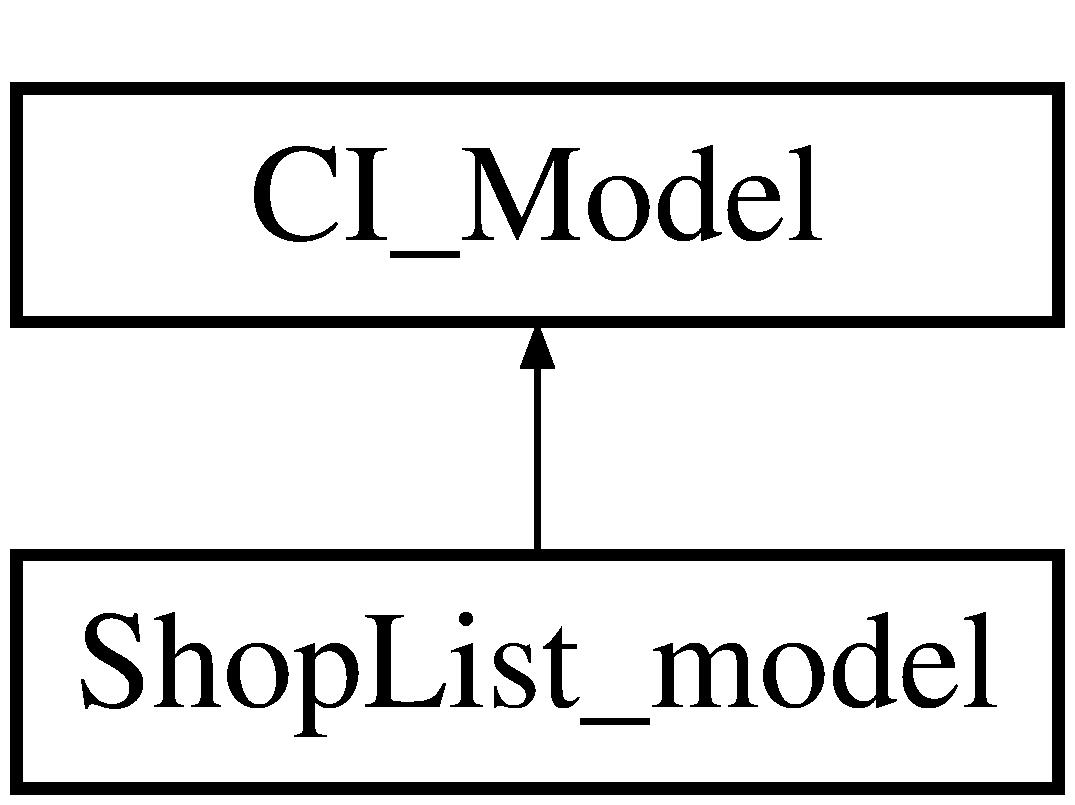
\includegraphics[height=2.000000cm]{class_shop_list__model}
\end{center}
\end{figure}
\subsection*{Public Member Functions}
\begin{DoxyCompactItemize}
\item 
\mbox{\Hypertarget{class_shop_list__model_ae033cd78c033b7cc3796a24994e451a5}\label{class_shop_list__model_ae033cd78c033b7cc3796a24994e451a5}} 
{\bfseries get\+Shops} (int \$id\+\_\+user)
\item 
\mbox{\Hypertarget{class_shop_list__model_a199cefde9fd328894e3498b1cd3ac37d}\label{class_shop_list__model_a199cefde9fd328894e3498b1cd3ac37d}} 
{\bfseries get\+All\+Shops} ()
\item 
\mbox{\Hypertarget{class_shop_list__model_a9d8bcfe6c594f4c9d148b67d2e3322ac}\label{class_shop_list__model_a9d8bcfe6c594f4c9d148b67d2e3322ac}} 
{\bfseries get\+Shop\+In} (string \$in)
\item 
\mbox{\Hypertarget{class_shop_list__model_aced1f7b553d96d232bb3493adde7c28f}\label{class_shop_list__model_aced1f7b553d96d232bb3493adde7c28f}} 
{\bfseries add\+Shop\+To\+User} (\$user\+\_\+id, \$shop\+\_\+name)
\end{DoxyCompactItemize}


The documentation for this class was generated from the following file\+:\begin{DoxyCompactItemize}
\item 
application/models/Shop\+List\+\_\+model.\+php\end{DoxyCompactItemize}

\hypertarget{class_shopping_list__model}{}\section{Shopping\+List\+\_\+model Class Reference}
\label{class_shopping_list__model}\index{Shopping\+List\+\_\+model@{Shopping\+List\+\_\+model}}
Inheritance diagram for Shopping\+List\+\_\+model\+:\begin{figure}[H]
\begin{center}
\leavevmode
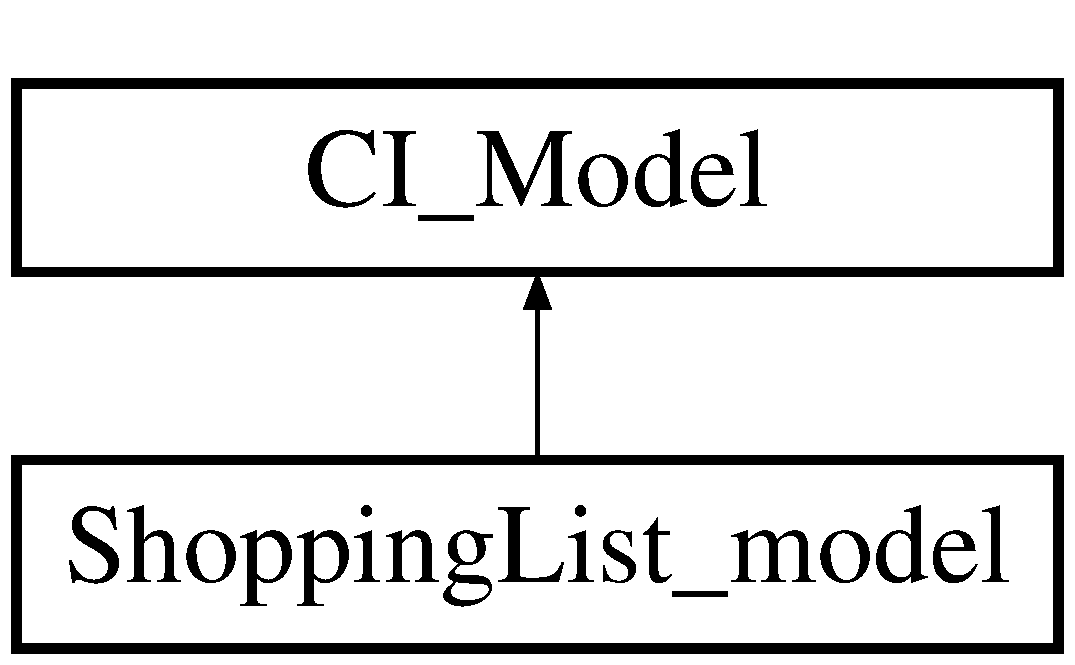
\includegraphics[height=2.000000cm]{class_shopping_list__model}
\end{center}
\end{figure}
\subsection*{Public Member Functions}
\begin{DoxyCompactItemize}
\item 
\hyperlink{class_shopping_list__model_af711613df11b7db405b82e41a00cbfcd}{create\+Empty\+List} (int \$id\+\_\+user)
\item 
\hyperlink{class_shopping_list__model_ae5bcc5afcc548c0e408eef17b3c7398f}{delete\+List} (int \$id\+\_\+list)
\item 
\hyperlink{class_shopping_list__model_a1e37654033d0e20491d3171e4c8a1aee}{get\+Lists} (int \$id)
\item 
\hyperlink{class_shopping_list__model_a5e244bd766fe003179871105026b35fa}{get\+List\+By\+Id} (int \$id)
\item 
\hyperlink{class_shopping_list__model_a51e2298ec742c4ef89fc2be60437a3dc}{set\+Name} (int \$id, string \$name)
\item 
\hyperlink{class_shopping_list__model_af2649dd00c4ca7db91511e2dce1b7a76}{get\+Products} (int \$id\+\_\+list)
\item 
\hyperlink{class_shopping_list__model_a1c9d4fb3435fef3e10b9aaaa8ba0a267}{get\+Products\+Like} (string \$name)
\item 
\hyperlink{class_shopping_list__model_ab632694703ad6ff436e878f20f1c1eee}{add\+Product\+To\+List} (int \$id\+\_\+list, string \$id\+\_\+product)
\item 
\hyperlink{class_shopping_list__model_a4d69ff874fe3d7cc49a9e49ae17295b1}{delete\+Product\+From\+List} (int \$id\+\_\+list, int \$id\+\_\+product)
\item 
\hyperlink{class_shopping_list__model_a95344ec0b769c9ecf4b423b54fb88c40}{get\+Product\+By\+Id} (int \$id\+\_\+prod)
\item 
\hyperlink{class_shopping_list__model_a8271bb7a9235c363295b640d4ba58a84}{set\+Amount} (int \$id\+\_\+list, int \$id\+\_\+product, int \$amount)
\item 
\hyperlink{class_shopping_list__model_a1c91e4d37b6cc18d9ffca1e9718213bb}{get\+Amount} (int \$id\+\_\+list, int \$id\+\_\+product)
\item 
\hyperlink{class_shopping_list__model_a4c9b3d77ee0eb69acead909068091079}{update\+Note} (int \$id\+\_\+list, string \$note)
\end{DoxyCompactItemize}


\subsection{Member Function Documentation}
\mbox{\Hypertarget{class_shopping_list__model_ab632694703ad6ff436e878f20f1c1eee}\label{class_shopping_list__model_ab632694703ad6ff436e878f20f1c1eee}} 
\index{Shopping\+List\+\_\+model@{Shopping\+List\+\_\+model}!add\+Product\+To\+List@{add\+Product\+To\+List}}
\index{add\+Product\+To\+List@{add\+Product\+To\+List}!Shopping\+List\+\_\+model@{Shopping\+List\+\_\+model}}
\subsubsection{\texorpdfstring{add\+Product\+To\+List()}{addProductToList()}}
{\footnotesize\ttfamily add\+Product\+To\+List (\begin{DoxyParamCaption}\item[{int}]{\$id\+\_\+list,  }\item[{string}]{\$id\+\_\+product }\end{DoxyParamCaption})}

Add a product to a specidied list

Return True/false if insered or not \mbox{\Hypertarget{class_shopping_list__model_af711613df11b7db405b82e41a00cbfcd}\label{class_shopping_list__model_af711613df11b7db405b82e41a00cbfcd}} 
\index{Shopping\+List\+\_\+model@{Shopping\+List\+\_\+model}!create\+Empty\+List@{create\+Empty\+List}}
\index{create\+Empty\+List@{create\+Empty\+List}!Shopping\+List\+\_\+model@{Shopping\+List\+\_\+model}}
\subsubsection{\texorpdfstring{create\+Empty\+List()}{createEmptyList()}}
{\footnotesize\ttfamily create\+Empty\+List (\begin{DoxyParamCaption}\item[{int}]{\$id\+\_\+user }\end{DoxyParamCaption})}

Creates an empty List for a specified user \mbox{\Hypertarget{class_shopping_list__model_ae5bcc5afcc548c0e408eef17b3c7398f}\label{class_shopping_list__model_ae5bcc5afcc548c0e408eef17b3c7398f}} 
\index{Shopping\+List\+\_\+model@{Shopping\+List\+\_\+model}!delete\+List@{delete\+List}}
\index{delete\+List@{delete\+List}!Shopping\+List\+\_\+model@{Shopping\+List\+\_\+model}}
\subsubsection{\texorpdfstring{delete\+List()}{deleteList()}}
{\footnotesize\ttfamily delete\+List (\begin{DoxyParamCaption}\item[{int}]{\$id\+\_\+list }\end{DoxyParamCaption})}

Delete a list with a specified id \mbox{\Hypertarget{class_shopping_list__model_a4d69ff874fe3d7cc49a9e49ae17295b1}\label{class_shopping_list__model_a4d69ff874fe3d7cc49a9e49ae17295b1}} 
\index{Shopping\+List\+\_\+model@{Shopping\+List\+\_\+model}!delete\+Product\+From\+List@{delete\+Product\+From\+List}}
\index{delete\+Product\+From\+List@{delete\+Product\+From\+List}!Shopping\+List\+\_\+model@{Shopping\+List\+\_\+model}}
\subsubsection{\texorpdfstring{delete\+Product\+From\+List()}{deleteProductFromList()}}
{\footnotesize\ttfamily delete\+Product\+From\+List (\begin{DoxyParamCaption}\item[{int}]{\$id\+\_\+list,  }\item[{int}]{\$id\+\_\+product }\end{DoxyParamCaption})}

Delete a product for a specified list \mbox{\Hypertarget{class_shopping_list__model_a1c91e4d37b6cc18d9ffca1e9718213bb}\label{class_shopping_list__model_a1c91e4d37b6cc18d9ffca1e9718213bb}} 
\index{Shopping\+List\+\_\+model@{Shopping\+List\+\_\+model}!get\+Amount@{get\+Amount}}
\index{get\+Amount@{get\+Amount}!Shopping\+List\+\_\+model@{Shopping\+List\+\_\+model}}
\subsubsection{\texorpdfstring{get\+Amount()}{getAmount()}}
{\footnotesize\ttfamily get\+Amount (\begin{DoxyParamCaption}\item[{int}]{\$id\+\_\+list,  }\item[{int}]{\$id\+\_\+product }\end{DoxyParamCaption})}

Get the amount of a specified product in a specified list \mbox{\Hypertarget{class_shopping_list__model_a5e244bd766fe003179871105026b35fa}\label{class_shopping_list__model_a5e244bd766fe003179871105026b35fa}} 
\index{Shopping\+List\+\_\+model@{Shopping\+List\+\_\+model}!get\+List\+By\+Id@{get\+List\+By\+Id}}
\index{get\+List\+By\+Id@{get\+List\+By\+Id}!Shopping\+List\+\_\+model@{Shopping\+List\+\_\+model}}
\subsubsection{\texorpdfstring{get\+List\+By\+Id()}{getListById()}}
{\footnotesize\ttfamily get\+List\+By\+Id (\begin{DoxyParamCaption}\item[{int}]{\$id }\end{DoxyParamCaption})}

Get a list by giving it id \mbox{\Hypertarget{class_shopping_list__model_a1e37654033d0e20491d3171e4c8a1aee}\label{class_shopping_list__model_a1e37654033d0e20491d3171e4c8a1aee}} 
\index{Shopping\+List\+\_\+model@{Shopping\+List\+\_\+model}!get\+Lists@{get\+Lists}}
\index{get\+Lists@{get\+Lists}!Shopping\+List\+\_\+model@{Shopping\+List\+\_\+model}}
\subsubsection{\texorpdfstring{get\+Lists()}{getLists()}}
{\footnotesize\ttfamily get\+Lists (\begin{DoxyParamCaption}\item[{int}]{\$id }\end{DoxyParamCaption})}

Get all lists of a specified user(id) \mbox{\Hypertarget{class_shopping_list__model_a95344ec0b769c9ecf4b423b54fb88c40}\label{class_shopping_list__model_a95344ec0b769c9ecf4b423b54fb88c40}} 
\index{Shopping\+List\+\_\+model@{Shopping\+List\+\_\+model}!get\+Product\+By\+Id@{get\+Product\+By\+Id}}
\index{get\+Product\+By\+Id@{get\+Product\+By\+Id}!Shopping\+List\+\_\+model@{Shopping\+List\+\_\+model}}
\subsubsection{\texorpdfstring{get\+Product\+By\+Id()}{getProductById()}}
{\footnotesize\ttfamily get\+Product\+By\+Id (\begin{DoxyParamCaption}\item[{int}]{\$id\+\_\+prod }\end{DoxyParamCaption})}

Return Product by its ID. \mbox{\Hypertarget{class_shopping_list__model_af2649dd00c4ca7db91511e2dce1b7a76}\label{class_shopping_list__model_af2649dd00c4ca7db91511e2dce1b7a76}} 
\index{Shopping\+List\+\_\+model@{Shopping\+List\+\_\+model}!get\+Products@{get\+Products}}
\index{get\+Products@{get\+Products}!Shopping\+List\+\_\+model@{Shopping\+List\+\_\+model}}
\subsubsection{\texorpdfstring{get\+Products()}{getProducts()}}
{\footnotesize\ttfamily get\+Products (\begin{DoxyParamCaption}\item[{int}]{\$id\+\_\+list }\end{DoxyParamCaption})}

Return products of a specified list \mbox{\Hypertarget{class_shopping_list__model_a1c9d4fb3435fef3e10b9aaaa8ba0a267}\label{class_shopping_list__model_a1c9d4fb3435fef3e10b9aaaa8ba0a267}} 
\index{Shopping\+List\+\_\+model@{Shopping\+List\+\_\+model}!get\+Products\+Like@{get\+Products\+Like}}
\index{get\+Products\+Like@{get\+Products\+Like}!Shopping\+List\+\_\+model@{Shopping\+List\+\_\+model}}
\subsubsection{\texorpdfstring{get\+Products\+Like()}{getProductsLike()}}
{\footnotesize\ttfamily get\+Products\+Like (\begin{DoxyParamCaption}\item[{string}]{\$name }\end{DoxyParamCaption})}

Return names of product like param. Used from Ajax request \mbox{\Hypertarget{class_shopping_list__model_a8271bb7a9235c363295b640d4ba58a84}\label{class_shopping_list__model_a8271bb7a9235c363295b640d4ba58a84}} 
\index{Shopping\+List\+\_\+model@{Shopping\+List\+\_\+model}!set\+Amount@{set\+Amount}}
\index{set\+Amount@{set\+Amount}!Shopping\+List\+\_\+model@{Shopping\+List\+\_\+model}}
\subsubsection{\texorpdfstring{set\+Amount()}{setAmount()}}
{\footnotesize\ttfamily set\+Amount (\begin{DoxyParamCaption}\item[{int}]{\$id\+\_\+list,  }\item[{int}]{\$id\+\_\+product,  }\item[{int}]{\$amount }\end{DoxyParamCaption})}

Set the amount of a specified product in a specified list \mbox{\Hypertarget{class_shopping_list__model_a51e2298ec742c4ef89fc2be60437a3dc}\label{class_shopping_list__model_a51e2298ec742c4ef89fc2be60437a3dc}} 
\index{Shopping\+List\+\_\+model@{Shopping\+List\+\_\+model}!set\+Name@{set\+Name}}
\index{set\+Name@{set\+Name}!Shopping\+List\+\_\+model@{Shopping\+List\+\_\+model}}
\subsubsection{\texorpdfstring{set\+Name()}{setName()}}
{\footnotesize\ttfamily set\+Name (\begin{DoxyParamCaption}\item[{int}]{\$id,  }\item[{string}]{\$name }\end{DoxyParamCaption})}

Set name of a specified list \mbox{\Hypertarget{class_shopping_list__model_a4c9b3d77ee0eb69acead909068091079}\label{class_shopping_list__model_a4c9b3d77ee0eb69acead909068091079}} 
\index{Shopping\+List\+\_\+model@{Shopping\+List\+\_\+model}!update\+Note@{update\+Note}}
\index{update\+Note@{update\+Note}!Shopping\+List\+\_\+model@{Shopping\+List\+\_\+model}}
\subsubsection{\texorpdfstring{update\+Note()}{updateNote()}}
{\footnotesize\ttfamily update\+Note (\begin{DoxyParamCaption}\item[{int}]{\$id\+\_\+list,  }\item[{string}]{\$note }\end{DoxyParamCaption})}

Update note for a product in a specified list 

The documentation for this class was generated from the following file\+:\begin{DoxyCompactItemize}
\item 
application/models/Shopping\+List\+\_\+model.\+php\end{DoxyCompactItemize}

\hypertarget{class_user__model}{}\section{User\+\_\+model Class Reference}
\label{class_user__model}\index{User\+\_\+model@{User\+\_\+model}}
Inheritance diagram for User\+\_\+model\+:\begin{figure}[H]
\begin{center}
\leavevmode
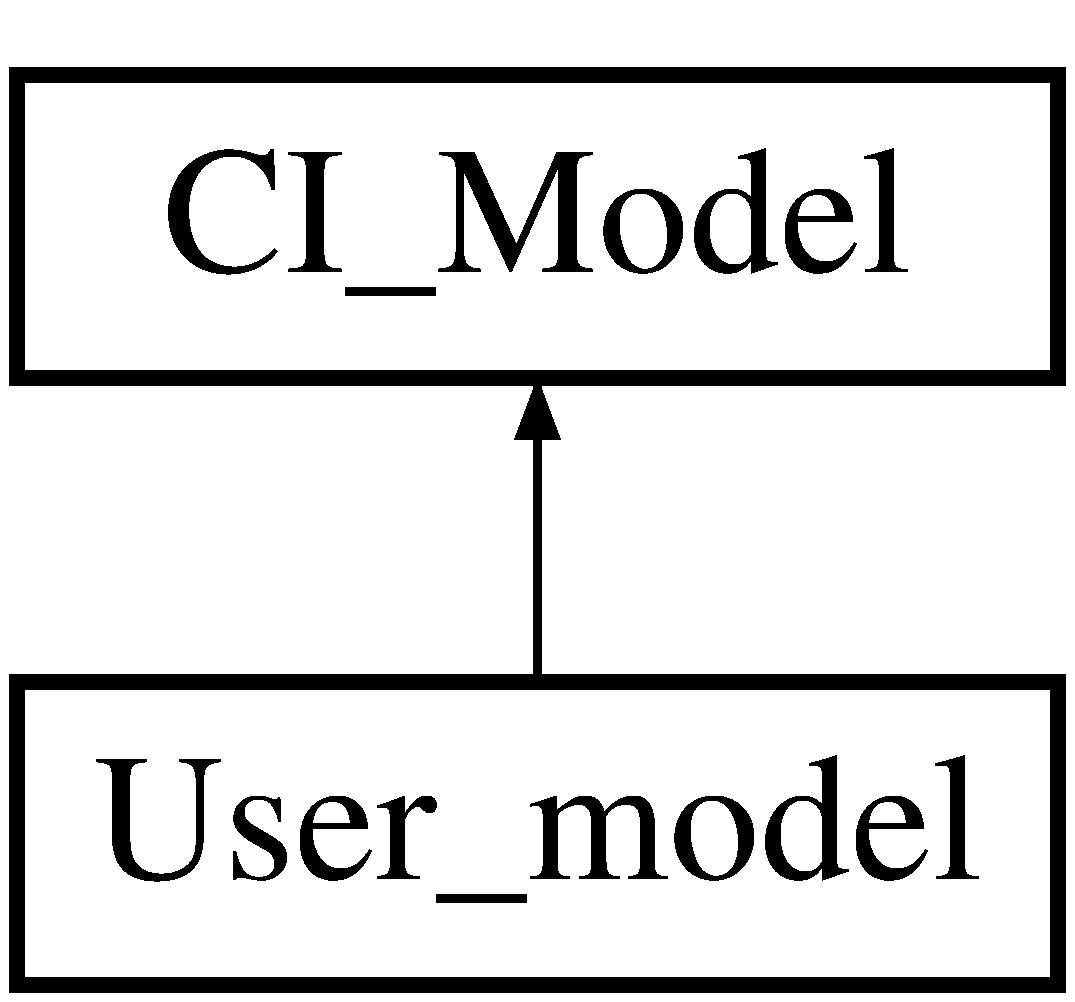
\includegraphics[height=2.000000cm]{class_user__model}
\end{center}
\end{figure}
\subsection*{Public Member Functions}
\begin{DoxyCompactItemize}
\item 
\hyperlink{class_user__model_ae3c97430ddfbb524172fe62687493762}{id} (\$login)
\item 
\hyperlink{class_user__model_abdfab30e2e8e5562e761a2228af18c3b}{add\+User} (\$user)
\item 
\hyperlink{class_user__model_ad956699f65b6a767bdf9ce2d251633b2}{valid\+\_\+infos\+\_\+connexion} (\$login, \$password)
\item 
\mbox{\Hypertarget{class_user__model_a3204c52d23a035d36787a16d82db1333}\label{class_user__model_a3204c52d23a035d36787a16d82db1333}} 
{\bfseries login\+\_\+existe} (\$str)
\item 
\mbox{\Hypertarget{class_user__model_a4084ea600d7d896ff95d9248a7a25616}\label{class_user__model_a4084ea600d7d896ff95d9248a7a25616}} 
{\bfseries email\+\_\+existe} (\$str)
\item 
\hyperlink{class_user__model_a40e51a5c6fc819d5c0f2e678a124d60e}{infos} (\$login)
\item 
\hyperlink{class_user__model_a1e8eb7d545bc221a640bffdebf063e3e}{modifier\+\_\+mdp} (\$login, \$password)
\item 
\hyperlink{class_user__model_af67174e59f20721772935e2318be5e4a}{ajouter\+\_\+ami} (\$login\+\_\+donne\+\_\+acces, \$login\+\_\+a\+\_\+acces)
\item 
\hyperlink{class_user__model_a778aaa6e58fc26c945fffba005867051}{obtenir\+\_\+amis} (\$login, \$a\+\_\+accepter=F\+A\+L\+SE)
\item 
\mbox{\Hypertarget{class_user__model_a30fbd50d8c0d3312dee36d8de939ebca}\label{class_user__model_a30fbd50d8c0d3312dee36d8de939ebca}} 
{\bfseries obtenir\+\_\+notifications} (\$login)
\item 
\hyperlink{class_user__model_a6bac1a29e9d14095868f8d38b2a814b2}{supprimer\+\_\+ami} (\$login1, \$login2)
\item 
\hyperlink{class_user__model_a54a357608c9913546f397fad6270e4fb}{sont\+\_\+amis} (\$login1, int \$id2, \$access=false)
\end{DoxyCompactItemize}


\subsection{Member Function Documentation}
\mbox{\Hypertarget{class_user__model_abdfab30e2e8e5562e761a2228af18c3b}\label{class_user__model_abdfab30e2e8e5562e761a2228af18c3b}} 
\index{User\+\_\+model@{User\+\_\+model}!add\+User@{add\+User}}
\index{add\+User@{add\+User}!User\+\_\+model@{User\+\_\+model}}
\subsubsection{\texorpdfstring{add\+User()}{addUser()}}
{\footnotesize\ttfamily add\+User (\begin{DoxyParamCaption}\item[{}]{\$user }\end{DoxyParamCaption})}

Adds the specified user in the database \mbox{\Hypertarget{class_user__model_af67174e59f20721772935e2318be5e4a}\label{class_user__model_af67174e59f20721772935e2318be5e4a}} 
\index{User\+\_\+model@{User\+\_\+model}!ajouter\+\_\+ami@{ajouter\+\_\+ami}}
\index{ajouter\+\_\+ami@{ajouter\+\_\+ami}!User\+\_\+model@{User\+\_\+model}}
\subsubsection{\texorpdfstring{ajouter\+\_\+ami()}{ajouter\_ami()}}
{\footnotesize\ttfamily ajouter\+\_\+ami (\begin{DoxyParamCaption}\item[{}]{\$login\+\_\+donne\+\_\+acces,  }\item[{}]{\$login\+\_\+a\+\_\+acces }\end{DoxyParamCaption})}

Adds a friend. More precisely, the second specified user gets access to the first specified user\textquotesingle{}s lists. \mbox{\Hypertarget{class_user__model_ae3c97430ddfbb524172fe62687493762}\label{class_user__model_ae3c97430ddfbb524172fe62687493762}} 
\index{User\+\_\+model@{User\+\_\+model}!id@{id}}
\index{id@{id}!User\+\_\+model@{User\+\_\+model}}
\subsubsection{\texorpdfstring{id()}{id()}}
{\footnotesize\ttfamily id (\begin{DoxyParamCaption}\item[{}]{\$login }\end{DoxyParamCaption})}

Returns user id \mbox{\Hypertarget{class_user__model_a40e51a5c6fc819d5c0f2e678a124d60e}\label{class_user__model_a40e51a5c6fc819d5c0f2e678a124d60e}} 
\index{User\+\_\+model@{User\+\_\+model}!infos@{infos}}
\index{infos@{infos}!User\+\_\+model@{User\+\_\+model}}
\subsubsection{\texorpdfstring{infos()}{infos()}}
{\footnotesize\ttfamily infos (\begin{DoxyParamCaption}\item[{}]{\$login }\end{DoxyParamCaption})}

Returns user\textquotesingle{}s information (login, mail, name and first name). \mbox{\Hypertarget{class_user__model_a1e8eb7d545bc221a640bffdebf063e3e}\label{class_user__model_a1e8eb7d545bc221a640bffdebf063e3e}} 
\index{User\+\_\+model@{User\+\_\+model}!modifier\+\_\+mdp@{modifier\+\_\+mdp}}
\index{modifier\+\_\+mdp@{modifier\+\_\+mdp}!User\+\_\+model@{User\+\_\+model}}
\subsubsection{\texorpdfstring{modifier\+\_\+mdp()}{modifier\_mdp()}}
{\footnotesize\ttfamily modifier\+\_\+mdp (\begin{DoxyParamCaption}\item[{}]{\$login,  }\item[{}]{\$password }\end{DoxyParamCaption})}

Function used to change the user\textquotesingle{}s password. \mbox{\Hypertarget{class_user__model_a778aaa6e58fc26c945fffba005867051}\label{class_user__model_a778aaa6e58fc26c945fffba005867051}} 
\index{User\+\_\+model@{User\+\_\+model}!obtenir\+\_\+amis@{obtenir\+\_\+amis}}
\index{obtenir\+\_\+amis@{obtenir\+\_\+amis}!User\+\_\+model@{User\+\_\+model}}
\subsubsection{\texorpdfstring{obtenir\+\_\+amis()}{obtenir\_amis()}}
{\footnotesize\ttfamily obtenir\+\_\+amis (\begin{DoxyParamCaption}\item[{}]{\$login,  }\item[{}]{\$a\+\_\+accepter = {\ttfamily FALSE} }\end{DoxyParamCaption})}

Accept or delete a \char`\"{}friend invitation\char`\"{}. \mbox{\Hypertarget{class_user__model_a54a357608c9913546f397fad6270e4fb}\label{class_user__model_a54a357608c9913546f397fad6270e4fb}} 
\index{User\+\_\+model@{User\+\_\+model}!sont\+\_\+amis@{sont\+\_\+amis}}
\index{sont\+\_\+amis@{sont\+\_\+amis}!User\+\_\+model@{User\+\_\+model}}
\subsubsection{\texorpdfstring{sont\+\_\+amis()}{sont\_amis()}}
{\footnotesize\ttfamily sont\+\_\+amis (\begin{DoxyParamCaption}\item[{}]{\$login1,  }\item[{int}]{\$id2,  }\item[{}]{\$access = {\ttfamily false} }\end{DoxyParamCaption})}

Returns T\+R\+UE if the specified users are friends. \mbox{\Hypertarget{class_user__model_a6bac1a29e9d14095868f8d38b2a814b2}\label{class_user__model_a6bac1a29e9d14095868f8d38b2a814b2}} 
\index{User\+\_\+model@{User\+\_\+model}!supprimer\+\_\+ami@{supprimer\+\_\+ami}}
\index{supprimer\+\_\+ami@{supprimer\+\_\+ami}!User\+\_\+model@{User\+\_\+model}}
\subsubsection{\texorpdfstring{supprimer\+\_\+ami()}{supprimer\_ami()}}
{\footnotesize\ttfamily supprimer\+\_\+ami (\begin{DoxyParamCaption}\item[{}]{\$login1,  }\item[{}]{\$login2 }\end{DoxyParamCaption})}

Delete friend. \mbox{\Hypertarget{class_user__model_ad956699f65b6a767bdf9ce2d251633b2}\label{class_user__model_ad956699f65b6a767bdf9ce2d251633b2}} 
\index{User\+\_\+model@{User\+\_\+model}!valid\+\_\+infos\+\_\+connexion@{valid\+\_\+infos\+\_\+connexion}}
\index{valid\+\_\+infos\+\_\+connexion@{valid\+\_\+infos\+\_\+connexion}!User\+\_\+model@{User\+\_\+model}}
\subsubsection{\texorpdfstring{valid\+\_\+infos\+\_\+connexion()}{valid\_infos\_connexion()}}
{\footnotesize\ttfamily valid\+\_\+infos\+\_\+connexion (\begin{DoxyParamCaption}\item[{}]{\$login,  }\item[{}]{\$password }\end{DoxyParamCaption})}

Verifies the login information of the user. Returns T\+R\+UE if the information is valid. 

The documentation for this class was generated from the following file\+:\begin{DoxyCompactItemize}
\item 
application/models/User\+\_\+model.\+php\end{DoxyCompactItemize}

%--- End generated contents ---

% Index
\backmatter
\newpage
\phantomsection
\clearemptydoublepage
\addcontentsline{toc}{chapter}{Index}
\printindex

\end{document}
